\documentclass{article}

% if you need to pass options to natbib, use, e.g.:
% \PassOptionsToPackage{numbers, compress}{natbib}
% before loading nips_2017
%
% to avoid loading the natbib package, add option nonatbib:
% \usepackage[nonatbib]{nips_2017}
%\usepackage{nips_2017}

\RequirePackage[l2tabu, orthodox]{nag}
\documentclass{article}

% FONTS
\usepackage[T1]{fontenc}

% Replace default Latin Modern typewriter with its proportional counterpart
% http://www.tug.dk/FontCatalogue/lmoderntypewriterprop/
\renewcommand*\ttdefault{lmvtt}


%%% OPTION 1 - Fourier Math + New Century Schoolbook + ParaType Sans

% % Import Fourier Math (this imposes its own New Century Schoolbook type)
% % http://www.ctan.org/tex-archive/fonts/fouriernc/
%\usepackage{fouriernc}
%\usepackage{amsmath}
% % Replace with TeX Gyre Schola version of New Century Schoolbook (must scale!)
% % http://www.tug.dk/FontCatalogue/tgschola/
%\usepackage[scale=0.92]{tgschola}
%\usepackage[scaled=0.88]{PTSans}

%% OPTION 2 - MathDesign Math + Bitstream Charter + ParaType Sans

% Import MathDesign (this brings along Bitstream Charter)
% http://www.ctan.org/tex-archive/fonts/mathdesign/
\usepackage[bitstream-charter]{mathdesign}
\usepackage{amsmath}
\usepackage[scaled=0.92]{PTSans}


% %%% OPTION 3 - MTPRO 2 Math + Termes Times + ParaType Sans

% \usepackage{tgtermes}
% \usepackage{amsmath}
% \usepackage[subscriptcorrection,
%             amssymbols,
%             mtpbb,
%             mtpcal,
%             nofontinfo  % suppresses all warnings
%            ]{mtpro2}
% \usepackage{scalefnt,letltxmacro}
% \LetLtxMacro{\oldtextsc}{\textsc}
% \renewcommand{\textsc}[1]{\oldtextsc{\scalefont{1.10}#1}}
% \usepackage[scaled=0.92]{PTSans}

% GEOMETRY
\usepackage[
  paper  = letterpaper,
  left   = 1.65in,
  right  = 1.65in,
  top    = 1.0in,
  bottom = 1.0in,
  ]{geometry}

% COLOR
\usepackage[usenames,dvipsnames]{xcolor}
\definecolor{shadecolor}{gray}{0.9}

% SPACING and TEXT
\usepackage[final,expansion=alltext]{microtype}
\usepackage[english]{babel}
\usepackage[parfill]{parskip}
\usepackage{afterpage}
\usepackage{framed}
\usepackage{verbatim}

%redefine the leftbar environment to accept a width and coloring options
\renewenvironment{leftbar}[1][\hsize]
{%
  \def\FrameCommand
  {%
    {\color{Gray}\vrule width 3pt}%
    \hspace{10pt}%
    %\hspace{0pt}\fboxsep=\FrameSep\colorbox{black!10}%
  }%
  \MakeFramed{\hsize#1\advance\hsize-\width\FrameRestore}%
}%
{\endMakeFramed}

% define a paragraph header function
\DeclareRobustCommand{\parhead}[1]{\textbf{#1}~}

% EDITING
% line numbering in left margin
\usepackage{lineno}
\renewcommand\linenumberfont{\normalfont
                             \footnotesize
                             \sffamily
                             \color{SkyBlue}}
% ragged paragraphs in right margin
\usepackage{ragged2e}
\DeclareRobustCommand{\sidenote}[1]{\marginpar{
                                    \RaggedRight
                                    \textcolor{Plum}{\textsf{#1}}}}
% paragraph counter in right margin
\newcommand{\parnum}{\bfseries\P\arabic{parcount}}
\newcounter{parcount}
\newcommand\p{%
    \stepcounter{parcount}%
    \leavevmode\marginpar[\hfill\parnum]{\parnum}%
}
% paragraph helper
%\DeclareRobustCommand{\PP}{\textcolor{Plum}{\P} }

% COUNTERS
\renewcommand{\labelenumi}{\color{black!67}{\arabic{enumi}.}}
\renewcommand{\labelenumii}{{\color{black!67}(\alph{enumii})}}
\renewcommand{\labelitemi}{{\color{black!67}\textbullet}}

% FIGURES
\usepackage{graphicx}
\usepackage[labelfont=bf]{caption}
\usepackage[format=hang]{subcaption}

% TABLES
\usepackage{booktabs}

% ALGORITHMS
\usepackage[algoruled]{algorithm2e}
\usepackage{listings}
\usepackage{fancyvrb}
\fvset{fontsize=\normalsize}

% BIBLIOGRAPHY
\usepackage{natbib}

% HYPERREF
\usepackage[colorlinks,linktoc=all]{hyperref}
\usepackage[all]{hypcap}
\hypersetup{citecolor=BurntOrange}
\hypersetup{linkcolor=MidnightBlue}
\hypersetup{urlcolor=MidnightBlue}

% CLEVEREF must come after HYPERREF
\usepackage[nameinlink]{cleveref}

% ACRONYMS
\usepackage[acronym,smallcaps,nowarn]{glossaries}
% \makeglossaries

% COLOR DEFINITIONS
\newcommand{\red}[1]{\textcolor{BrickRed}{#1}}
\newcommand{\orange}[1]{\textcolor{BurntOrange}{#1}}
\newcommand{\green}[1]{\textcolor{OliveGreen}{#1}}
\newcommand{\blue}[1]{\textcolor{MidnightBlue}{#1}}
\newcommand{\gray}[1]{\textcolor{black!60}{#1}}

% LISTINGS DEFINTIONS
\lstdefinestyle{mystyle}{
    commentstyle=\color{OliveGreen},
    keywordstyle=\color{BurntOrange},
    numberstyle=\tiny\color{black!60},
    stringstyle=\color{MidnightBlue},
    basicstyle=\ttfamily,
    breakatwhitespace=false,
    breaklines=true,
    captionpos=b,
    keepspaces=true,
    numbers=left,
    numbersep=5pt,
    showspaces=false,
    showstringspaces=false,
    showtabs=false,
    tabsize=2
}
\lstset{style=mystyle}

\DeclareRobustCommand{\mb}[1]{\ensuremath{\boldsymbol{\mathbf{#1}}}}
\DeclareRobustCommand{\KL}[2]{\ensuremath{\textrm{KL}\left(#1\;\|\;#2\right)}}

\newcommand{\supp}{\textrm{supp}}

\newcommand{\E}{\mathbb{E}}
\newcommand{\Var}{\mathbb{V}\textrm{ar}}

% Redundant with reals, naturals, below
\newcommand{\bbN}{\mathbb{N}}
\newcommand{\bbZ}{\mathbb{Z}}
\newcommand{\bbR}{\mathbb{R}}
\newcommand{\bbS}{\mathbb{S}}
\newcommand{\bbH}{\mathbb{H}}


\newcommand{\bA}{\boldsymbol{A}}
\newcommand{\bB}{\boldsymbol{B}}
\newcommand{\bC}{\boldsymbol{C}}
\newcommand{\bD}{\boldsymbol{D}}
\newcommand{\bE}{\boldsymbol{E}}
\newcommand{\bF}{\boldsymbol{F}}
\newcommand{\bG}{\boldsymbol{G}}
\newcommand{\bH}{\boldsymbol{H}}
\newcommand{\bI}{\boldsymbol{I}}
\newcommand{\bJ}{\boldsymbol{J}}
\newcommand{\bK}{\boldsymbol{K}}
\newcommand{\bL}{\boldsymbol{L}}
\newcommand{\bM}{\boldsymbol{M}}
\newcommand{\bN}{\boldsymbol{N}}
\newcommand{\bO}{\boldsymbol{O}}
\newcommand{\bP}{\boldsymbol{P}}
\newcommand{\bQ}{\boldsymbol{Q}}
\newcommand{\bR}{\boldsymbol{R}}
\newcommand{\bS}{\boldsymbol{S}}
\newcommand{\bT}{\boldsymbol{T}}
\newcommand{\bU}{\boldsymbol{U}}
\newcommand{\bV}{\boldsymbol{V}}
\newcommand{\bW}{\boldsymbol{W}}
\newcommand{\bX}{\boldsymbol{X}}
\newcommand{\bY}{\boldsymbol{Y}}
\newcommand{\bZ}{\boldsymbol{Z}}
\newcommand{\ba}{\boldsymbol{a}}
\newcommand{\bb}{\boldsymbol{b}}
\newcommand{\bc}{\boldsymbol{c}}
\newcommand{\bd}{\boldsymbol{d}}
\newcommand{\be}{\boldsymbol{e}}
\newcommand{\bbf}{\boldsymbol{f}}
\newcommand{\bg}{\boldsymbol{g}}
\newcommand{\bh}{\boldsymbol{h}}
\newcommand{\bi}{\boldsymbol{i}}
\newcommand{\bj}{\boldsymbol{j}}
\newcommand{\bk}{\boldsymbol{k}}
\newcommand{\bl}{\boldsymbol{l}}
\newcommand{\bbm}{\boldsymbol{m}}
\newcommand{\bn}{\boldsymbol{n}}
\newcommand{\bo}{\boldsymbol{o}}
\newcommand{\bp}{\boldsymbol{p}}
\newcommand{\bq}{\boldsymbol{q}}
\newcommand{\br}{\boldsymbol{r}}
\newcommand{\bs}{\boldsymbol{s}}
\newcommand{\bt}{\boldsymbol{t}}
\newcommand{\bu}{\boldsymbol{u}}
\newcommand{\bv}{\boldsymbol{v}}
\newcommand{\bw}{\boldsymbol{w}}
\newcommand{\bx}{\boldsymbol{x}}
\newcommand{\by}{\boldsymbol{y}}
\newcommand{\bz}{\boldsymbol{z}}

\newcommand{\balpha}{\boldsymbol{\alpha}}
\newcommand{\bbeta}{\boldsymbol{\beta}}
\newcommand{\boldeta}{\boldsymbol{\eta}}
\newcommand{\bkappa}{\boldsymbol{\kappa}}
\newcommand{\bgamma}{\boldsymbol{\gamma}}
\newcommand{\blambda}{\boldsymbol{\lambda}}
\newcommand{\bmu}{\boldsymbol{\mu}}
\newcommand{\bnu}{\boldsymbol{\nu}}
\newcommand{\brho}{\boldsymbol{\rho}}
\newcommand{\bphi}{\boldsymbol{\phi}}
\newcommand{\bpi}{\boldsymbol{\pi}}
\newcommand{\bpsi}{\boldsymbol{\psi}}
\newcommand{\bsigma}{\boldsymbol{\sigma}}
\newcommand{\btheta}{\boldsymbol{\theta}}
\newcommand{\bomega}{\boldsymbol{\omega}}
\newcommand{\bxi}{\boldsymbol{\xi}}
\newcommand{\bGamma}{\boldsymbol{\Gamma}}
\newcommand{\bLambda}{\boldsymbol{\Lambda}}
\newcommand{\bOmega}{\boldsymbol{\Omega}}
\newcommand{\bPhi}{\boldsymbol{\Phi}}
\newcommand{\bPi}{\boldsymbol{\Pi}}
\newcommand{\bPsi}{\boldsymbol{\Psi}}
\newcommand{\bSigma}{\boldsymbol{\Sigma}}
\newcommand{\bTheta}{\boldsymbol{\Theta}}
\newcommand{\bUpsilon}{\boldsymbol{\Upsilon}}
\newcommand{\bXi}{\boldsymbol{\Xi}}
\newcommand{\bepsilon}{\boldsymbol{\epsilon}}

\newcommand{\mcA}{\mathcal{A}}
\newcommand{\mcB}{\mathcal{B}}
\newcommand{\mcC}{\mathcal{C}}
\newcommand{\mcD}{\mathcal{D}}
\newcommand{\mcE}{\mathcal{E}}
\newcommand{\mcF}{\mathcal{F}}
\newcommand{\mcG}{\mathcal{G}}
\newcommand{\mcH}{\mathcal{H}}
\newcommand{\mcI}{\mathcal{I}}
\newcommand{\mcJ}{\mathcal{J}}
\newcommand{\mcK}{\mathcal{K}}
\newcommand{\mcL}{\mathcal{L}}
\newcommand{\mcM}{\mathcal{M}}
\newcommand{\mcN}{\mathcal{N}}
\newcommand{\mcO}{\mathcal{O}}
\newcommand{\mcP}{\mathcal{P}}
\newcommand{\mcQ}{\mathcal{Q}}
\newcommand{\mcR}{\mathcal{R}}
\newcommand{\mcS}{\mathcal{S}}
\newcommand{\mcT}{\mathcal{T}}
\newcommand{\mcU}{\mathcal{U}}
\newcommand{\mcV}{\mathcal{V}}
\newcommand{\mcW}{\mathcal{W}}
\newcommand{\mcX}{\mathcal{X}}
\newcommand{\mcY}{\mathcal{Y}}
\newcommand{\mcZ}{\mathcal{Z}}

\newcommand{\trans}{\mathsf{T}}
\newcommand{\naturals}{\mathbb{N}}
\newcommand{\reals}{\mathbb{R}}
\def\argmax{\operatornamewithlimits{arg\,max}}
\def\argmin{\operatornamewithlimits{arg\,min}}

\newcommand{\distNormal}{\mathcal{N}}
\newcommand{\distGamma}{\mathrm{Gamma}}
\newcommand{\distBernoulli}{\mathrm{Bern}}
\newcommand{\distBinomial}{\mathrm{Bin}}
\newcommand{\distCategorical}{\mathrm{Cat}}
\newcommand{\distDirichlet}{\mathrm{Dir}}
\newcommand{\distMultinomial}{\mathrm{Mult}}
\newcommand{\distPolyaGamma}{\mathrm{PG}}
\newcommand{\distMNIW}{\mathrm{MNIW}}
\newcommand{\distBeta}{\mathrm{Beta}}

\newcommand{\prt}[1]{\frac{\partial}{\partial #1}}
\newcommand{\deriv}[1]{\frac{\mathrm{d}}{\mathrm{d} #1}}


\newcommand{\TODO}[1]{\textcolor{red}{[TODO: #1]}}

\newcommand{\bbI}{\mathbb{I}}
\newcommand{\bbE}{\mathbb{E}}
\newcommand{\bone}{\boldsymbol{1}}
\newcommand{\bigO}{\mathcal{O}}
\newcommand{\iid}[1]{\stackrel{\text{iid}}{#1}}
\newcommand\indep{\protect\mathpalette{\protect\independenT}{\perp}}
\def\independenT#1#2{\mathrel{\rlap{$#1#2$}\mkern4mu{#1#2}}}
\DeclareMathOperator{\Skew}{Skew}
\DeclareMathOperator{\Symm}{Sym}
\DeclareMathOperator{\tr}{tr}

%\DeclareMathOperator{\KL}{KL}
\newcommand{\given}{\, | \,}

\DeclareMathOperator{\diag}{diag}
\let\vec\relax% Set equal to \relax so that LaTeX thinks it's not defined
\DeclareMathOperator{\vec}{vec}
\let\Re\relax
\DeclareMathOperator{\Re}{\textup{Re}}
\let\Im\relax
\DeclareMathOperator{\Im}{\textup{Im}}

% Backcompat: dif and diff both work
\newcommand*\dif{\mathop{}\!\mathrm{d}}
\newcommand*\diff{\mathop{}\!\mathrm{d}}


% !TEX root = template.tex

\newacronym{KL}{kl}{Kullback-Leibler}
\newacronym{ELBO}{elbo}{evidence lower bound}
\newacronym{SVI}{svi}{stochastic variational inference}
\newacronym{GMM}{gmm}{Gaussian mixture model}
\newacronym{LDA}{lda}{latent Dirichlet allocation}


\usepackage{makecell}
\usepackage{blindtext}
\DeclareRobustCommand{\parhead}[1]{\textbf{#1}~}



% to compile a camera-ready version, add the [final] option, e.g.:
\usepackage[final]{nips_2017}
\usepackage{graphicx}
\usepackage[utf8]{inputenc} % allow utf-8 input
\usepackage[T1]{fontenc}    % use 8-bit T1 fonts
\usepackage{hyperref}       % hyperlinks
\usepackage{url}            % simple URL typesetting
\usepackage{booktabs}       % professional-quality tables
\usepackage{amsfonts}       % blackboard math symbols
\usepackage{nicefrac}       % compact symbols for 1/2, etc.
\usepackage{microtype}      % microtypography

\title{Toward Bayesian permutation inference for \\identifying neurons in \textit{C. elegans}.}

% The \author macro works with any number of authors. There are two
% commands used to separate the names and addresses of multiple
% authors: \And and \AND.
%
% Using \And between authors leaves it to LaTeX to determine where to
% break the lines. Using \AND forces a line break at that point. So,
% if LaTeX puts 3 of 4 authors names on the first line, and the last
% on the second line, try using \AND instead of \And before the third
% author name.

\author{
  Gonzalo Mena \thanks{The two authors equally contributed} \\
  Columbia University\\
   \And
  Scott Linderman  $^{*}$ \\
  Columbia University \\
  %% Address \\
  %% \texttt{email} \\
   \AND
  David Belanger\\
  Google Brain \\
  %% Address \\
  %% \texttt{email} \\
  \And
  Jasper Snoek\\
  Google Brain \\
  \And
  John Cunningham\\
  Columbia Univeristy \\
   \And
  Liam Paninski \\
  Columbia University\\
  %% Address \\
  %% \texttt{email} \\
}

\begin{document}
% \nipsfinalcopy is no longer used

\maketitle

\begin{abstract}
  The nematode C. elegans is a unique model organism for
  neuroscientists as its connectome, or neural wiring diagram, has
  been known for at least three decades. Despite this knowledge, an
  understanding of the functional significance of these synaptic
  connections has remained elusive. Now several groups can routinely
  image the activity of a large fraction of neurons in the head of the
  worm, providing a unique opportunity to probe this organism. We
  propose a hierarchical Bayesian framework that combines strong prior
  information with data from many experiments to estimate posteriors
  over the functional connectivity weights. However, first we must
  clear a significant hurdle: in many cases we are not sure
  exactly which neurons are being imaged, so to combine information
  across experiments we must solve a matching, or permutation
  inference, problem. In this work we introduce new variational
  methods designed for joint inference of connectivity weights and
  neural identity. Working with actual permutations would involve
  evaluating and differentiating an intractable partition function. As
  an alternative, we build upon recent continuous relaxation
  techniques \citep{Jang2016, Maddison2016}, extending them from the
  original case of the probability simplex, to the Birkhoff polytope,
  the convex hull of permutation matrices. We test our method with
  simulated data from the true connectome and show that our approach
  outperforms many alternatives in this synthetic neural identification task.
\end{abstract}



\section{Introduction}
The nematode \textit{C. elegans} plays a special role as a model
organism in neuroscience since its neural network is stereotyped from
animal to animal and its complete neural wiring diagram is
known~\citep{varshney2011structural}.  Modern calcium imaging
technology enables measurements of hundreds of these neurons
simultaneously \citep{Kato2015, nguyen2016whole}. The time is
right to employ modern statistical methods to learn about the
functional connectome in this system.

\begin{figure*}[t]
  \centering
  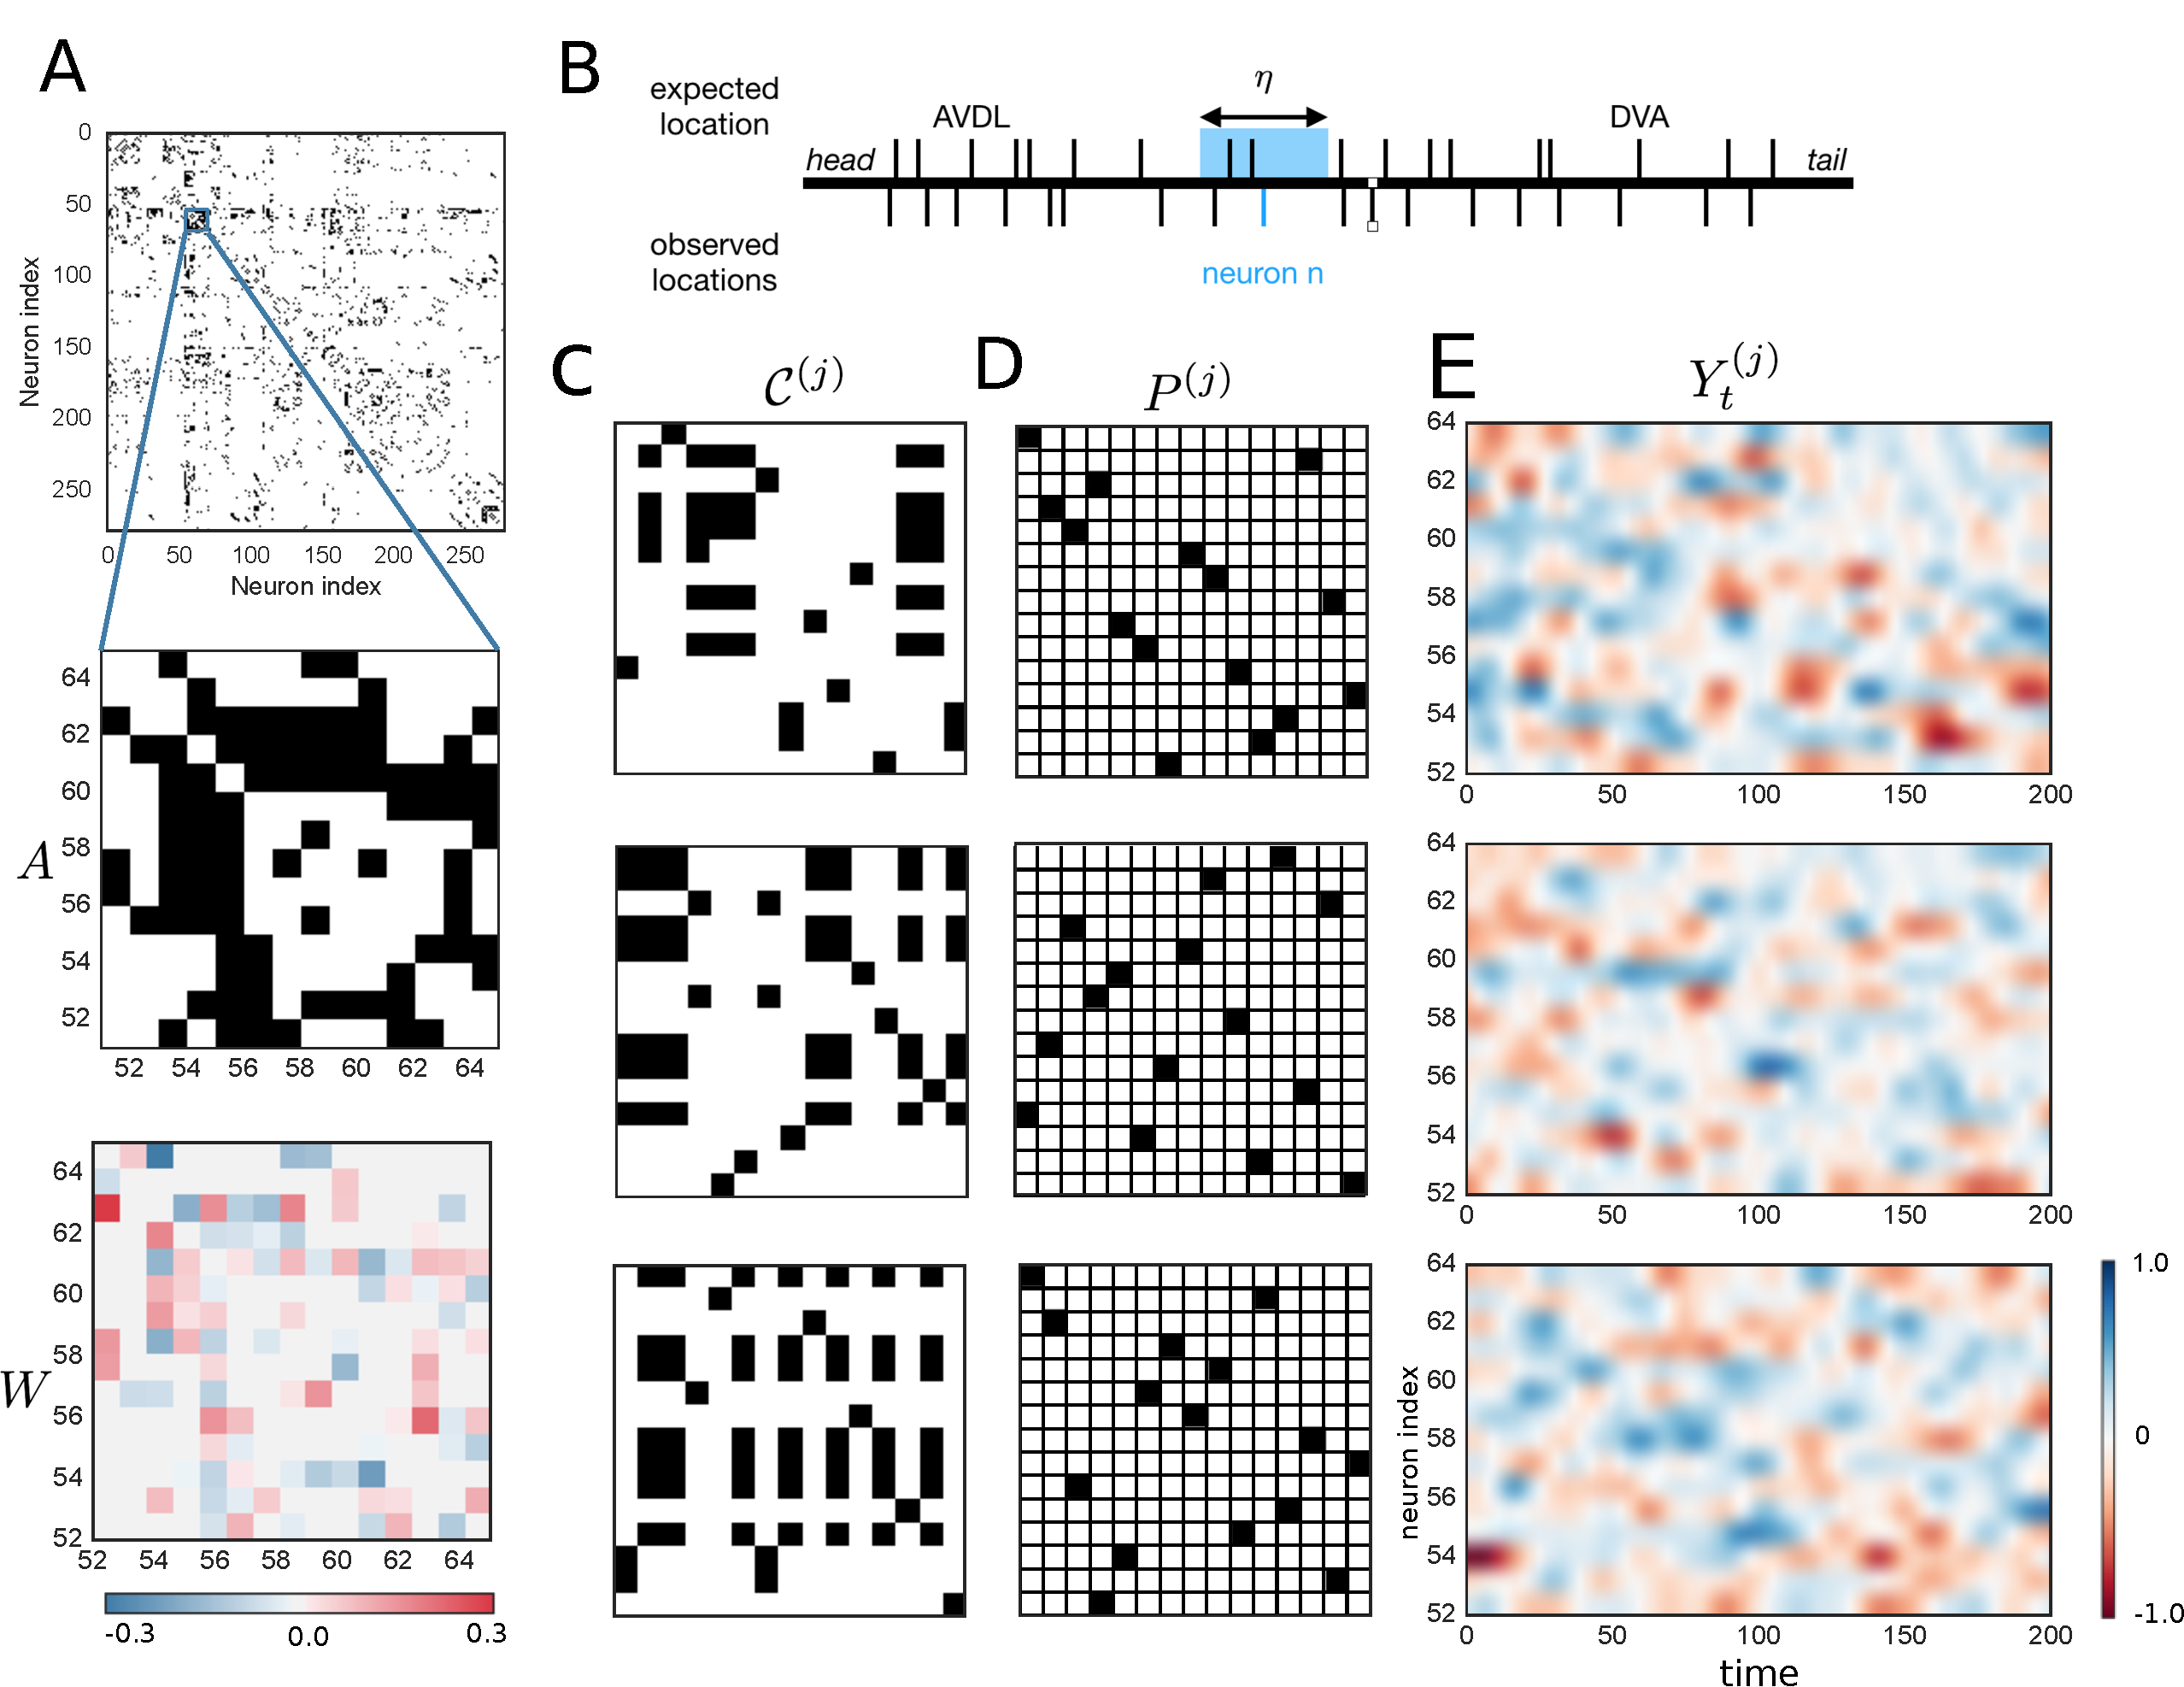
\includegraphics[width=5in]{Figure1.pdf} 
  \caption{\textit{Hierarchical Bayesian framework}.  \textbf{A} We
    are given the actual adjacency matrix $A$ from
    \citep{varshney2011structural}. The full matrix is shown (top)
    along with a zoom-in to 14 neurons (center).  We wish to infer the
    corresponding weight matrix~$W$, an example of which is shown
    below.  \textbf{B} We also know the typical locations of the
    neurons \citep{white1986structure,wormatlas}. Given observed
    locations, we constrain possible assignments to neuron identities
    within~$\eta$ of the observed location.  \textbf{C} These
    constraints are represented as a matrix $\mathcal{C}^{(j)}$ for
    worm~$j$ which specifies possible assignments of observed neurons
    to known identities. This illustration shows three worms.
    \textbf{D} To infer the weights, we must first infer the
    permutation $P^{(j)}$ that matches the observed neurons in
    worm~$j$ to the set of known identities.  \textbf{E} The observed
    data is a matrix~$Y^{(j)}$ whose rows are ordered according to the
    order in which neurons were observed in that worm.  The
    permutation matrix maps this to the canonical ordering of the
    adjacency and weight matrices. Given~$\{Y^{(j)}\}_{j=1}^J$
    and~$A$, we infer~$\{P^{(j)}\}_{j=1}^J$ and~$W$.}
  \vspace{-1em}
\label{fig:1}
\end{figure*}

Ultimately, we are interested in the dynamical system that governs how
neural activity evolves given its history and sensory inputs.
Bayesian methods are ideally suited to this goal, allowing us to
represent hierarchical probabilistic structures and integrate our
prior knowledge about the connectome, the locations of neurons, etc.
Bayesian learning and inference in dynamical systems with MCMC methods
is well-studied, even for complicated
models~\citep{Freitas2001,Paninski2010}. Furthermore, hierarchical
models to incorporate information from many worms are easily
constructed in a Bayesian framework~\citep{Gelman2014}.

However, our efforts to integrate information across worms are
complicated by a major hurdle: in practice, associating recorded
traces to neuron names is a painstaking, manual process.
Experimenters consider the location of the neuron along with its
pattern of activity to perform this matching, but the process is
laborious and the results are prone to error.  Without neuron names,
we cannot represent recordings canonically or learn about how one
neuron influences another. This technical problem prevents the
automatic use of hierarchical methods.

We present a method that aims to overcome this hurdle by incorporating
inference over permutations that match observed neurons
\textit{(neuron 1, neuron 2, ..., neuron~$N$)} to known names
\textit{(AVAL, AVAR, ..., SMDR)}.  Once the observed neurons have been
mapped to canonical names, we can learn about the shared dynamical
system. We focus on a simple linear autoregressive
model for neural dynamics,
\begin{align}
  \widetilde{Y}_t^{(j)} &= (W \odot A) \widetilde{Y}_{t-1}^{(j)} + \epsilon_t^{(j)},
\end{align}
where~$W \in \reals^{N \times N}$ is the weight matrix we wish to infer;
$A \in \{0,1\}^{N \times N}$ is the known adjacency matrix or connectome;
$\odot$ denotes element-wise multiplication;
$\epsilon_t^{(j)} \sim \distNormal(0, \sigma^2 I)$;
and~$\widetilde{Y}_t^{(j)} \in \reals^N$ is the measured neural activity
at time~$t$ in worm~$j$.  The catch is that~$\widetilde{Y}_t^{(j)}$ is
assumed to be in canonical order; i.e. in the same order as the rows and
columns of~$W$ and~$A$. We actually observe,
\begin{align}
  Y_t^{(j)} &= P^{(j)} \widetilde{Y}_t^{(j)},
\end{align}
vectors that are permuted by matrix~$P^{(j)}$. In order to learn about~$W$,
we must also infer the permutation matrices. We place a Gaussian prior on~$W$.

The permutation matrices are constrained by side
information. Specifically, we use neural position along the worm's
body to constrain the possible neural identities for a given recorded
neuron. We only allow an observed neuron to be mapped to a known
identity if the observed location is within~$\eta$ of the expected
location.  This is illustrated in Fig.~\ref{fig:1}B. We represent
these constraints with the matrix~$\mathcal{C}^{(j)}$ so that
$\mathcal{C}^{(j)}_{mn}=1$ if and only if observed neuron $m$ is
within~$\eta$ of canonical neuron $n$'s expected location.  An
example is shown in Figure \ref{fig:1}C. We let~$P^{(j)}$ have a
uniform prior over the set of matrices allowable under the given
constraints.

We need to perform posterior inference of $p(\{W,P^{(j)}\} \given A, \{Y^{(j)}\})$.
MCMC with simple Metropolis-Hastings proposals is straightforward, but
we found this mixed poorly in practice. Motivated by recent advances
in automatic variational inference \citep{Blei2017}, we considered
ways of extending this technique to permutation inference.  In Section
\ref{sec:VI} we detail our VI formulation and summarize the methods we
developed. Then in Section \ref{sec:results} we show that these
methods outperform alternatives.

\section{New methods for variational inference of latent permutations}
\label{sec:VI}
Consider a latent variable model determined by a prior over the latent
$z \sim p(z)$ and a likelihood $p(y \given z)$ for the observed data $y$. In
the VI framework, we approximate the intractable 
posterior $p(z \given y)$ with the distribution~$q \in \mcQ$
that best approximates the posterior. For tractability, we assume~$\mcQ$ 
is indexed by a parameter~$\nu$; i.e.~$\mcQ = \{q(z; \nu): \nu \in \mcV\}$.
The approximation is typically assessed by the Kullback-Leibler (KL) divergence between the true posterior and variational approximation.
% \begin{align}
%   \nu^* &= \argmin_{\nu \in \mcV}
%           \mathrm{KL} \left(q(z; \nu )  \, \|  \,  p(z \given y)\right).
% \end{align}
Minimizing the KL divergence is equivalent to maximizing the \emph{evidence lower bound} (ELBO)
\begin{align}
  \label{eq:elbo}
  \mcL(\nu) \triangleq  \E_{q(z;\nu)}[\log p(y|z)]
  - \mathrm{KL}(q(z;\nu)\, \| \,  p(z)),
\end{align}
with respect to~$\nu$.  We typically maximize equation~\eqref{eq:elbo}
with stochastic optimization methods \citep{Kushner1987}:
specifically, we approximate the expectations in~\eqref{eq:elbo} with
Monte Carlo estimates and optimize the ELBO with stochastic gradient
ascent. One critical component is the choice of the Monte Carlo
approximation. Perhaps the most common choice is through the so called
\emph{score function estimator}. Unfortunately,
this estimator, also referred to as REINFORCE \citep{Williams1992},
cannot be applied to permutations, since it involves the evaluation
and differentiation of a likelihood which is intractable for any
non-trivial distribution over permutations (computing the partition
function involves a summation over~$N!$ terms).
 
The reparameterization trick \cite{Kingma2013} offers an appealing
alternative. If~$z$ can be written as a differentiable function of a
noise distribution and the parameters---i.e. if for certain $f$ and
$\xi\sim p(\xi)$ one has $z=f(\xi,\nu)$---then we can write the
expectation with respect to~$q(z)$ as an expectation with respect
to~$p(\xi)$ and bring the gradient inside the expectation.  In the
case of discrete random variables a reparameterization always exists
and it is given by the \emph{Gumbel trick}
\citep{Papandreou2011}, which states that one can sample
from any discrete distribution by perturbing each potential with
Gumbel i.i.d noise, and then finding the configuration with the
maximum value. Unfortunately, the underlying $f$ to this
reparameterization is the non-differentiable $\argmax$ operator,
precluding the use of gradient descent methods.

\citet{Jang2016} and \citet{Maddison2016} proposed a solution to this
problem, replacing the $\argmax$ by a temperature-dependent softmax
approximation, which in the limit converges to the original
$\argmax$. By combining the Gumbel trick with the softmax
approximation, they conceived the \emph{Concrete} or
\emph{Gumbel-Softmax} distribution, and obtained explicit distribution
formulae. Then, they showed how to perform variational inference in
discrete latent variable models using the reparameterization trick and
gradient descent. They replaced the original ELBO with a surrogate
appropriate for their continuous relaxation. The method works well if 
the temperature is chosen in a reasonable range: not too high, to avoid
degenerate distributions on the simplex; but also not too low, to
limit the variance the gradients.

We developed three methods for extending the Gubmel-softmax method to
permutations. We name then \emph{stick-breaking}, \emph{rounding} and
\emph{Gumbel-Sinkhorn} methods. We refer the reader to sections 3.1
and 3.2 of \cite{Linderman2017} and section 4 of
\cite{Anonymous2018learning} for details, respectively. Here we
briefly summarize them: the primary geometric object is the Birkhoff
polytope, the convex hull of permutation matrices, and the analog of
the probability simplex in the discrete case. In the stick-breaking
method, we generalize the standard construction on the simplex to
stick-breaking of the Birkhoff polytope. We show how to consistently
``break the stick'' while satisfying both the row and column
constraints that characterize a doubly stochastic matrix. For the
rounding construction, we start with a noise distribution and force it
to be close to permutation matrices by rounding them towards the
extreme-points of the Birkhoff polytope (i.e. permutation
matrices). Finally, for the Gumbel-Sinkhorn method we notice that the
so-called \emph{Sinkhorn operator}, or infinite and successive row and
column normalization of a matrix, is a natural extension of the
softmax operator. With this, we introduce the Gumbel-Sinkhorn
distribution, which approximates the sampling of a discrete
distribution over permutations. Importantly, while stick-breaking and
rounding yield explicit densities, Gumbel-Sinkhorn does not. However,
there are ways to circumvent this difficulty, and overall we observe
the latter performs the best.

\section{Results}
\label{sec:results}

\begin{table}[t]
     \caption{Accuracy in the C.elegans neural identification problem, for varying mean number of candidate neurons (10, 30, 45, 60) and number of worms.}
   \label{table:celeganssup}

   \centering
  \begin{tabular}{lllllllllll}
    & \multicolumn{2}{c}{10} & \multicolumn{2}{c}{30} &   \multicolumn{2}{c}{45} & \multicolumn{2}{c}{60} \\
    \cmidrule(lr){2-3} \cmidrule(lr){4-5} \cmidrule(lr){6-7} \cmidrule(lr){8-9}
& 1 worm & 4 worms & 1 Worm & 4 worms & 1 worm & 4 worms & 1 worms & 4 worms \\
    \midrule 
    NAIVE VI &.34 & .32 & .16 & .16 & .13 & .12 & .11 & .12 \\
   MAP   & .34 & .32  &.17 &.17& .14 & .13 & .13 & .12 \\
    MCMC   & .34 & .65  &.18 &.28& .14 & .17 & .13 & .15 \\
      %\makecell[l]{Gumbel-Sinkhorn \\ (no regularization)} 
     % &.77 & .92 & \textbf{.4} & .64 &  .25 & .44 & .21 & .39 \\
       %Rounding  (VI) &   .77  & .93 &  .33 &\textbf{.7} &  .18 & .48 & .17 & .37 \\
    VI   & \textbf{.79} & \textbf{.94} & \textbf{.4} & \textbf{.69} & \textbf{.25}&  \textbf{.51} & \textbf{.21} & \textbf{.44}\\
 
    \bottomrule
  \end{tabular}
\end{table}


\begin{table}[t]
  \caption{Accuracy in inferring true neural identity for different of
    proportion of known neurons and $\eta$.
  }%\todo[inline]{Gonzalo: Tell the reader what they should take away
   %from these results.  It seems like this significantly outperforms
   %Linderman et al. when there is significantly less data.  Also,
   %with more data the differences don't necessarily seem that
   %significant.  Why is that the case?  What makes this method better
   %in some circumstances than that one?}}
   \label{table:celegans}
   \centering
   \begin{tabular}{lllllllll}
    & \multicolumn{2}{c}{40.\%} & \multicolumn{2}{c}{30.\%} & \multicolumn{2}{c}{20.\%} & \multicolumn{2}{c}{10.\%}\\
    \cmidrule(lr){2-3} \cmidrule(lr){4-5} \cmidrule(lr){6-7} \cmidrule(lr){8-9}
    & $\eta=0.1$ & $\eta=0.2$ & $\eta=0.1$ & $\eta=0.2$  & $\eta=0.1$ & $\eta=0.2$  & $\eta=0.1$ & $\eta=0.2$ \\
    \midrule 
    Naive VI & .43 & .41 & .33 & .31 & .23 & .22 & .12 & .1 \\
    MAP & .42 & .41  &.33 &.32& .23 & .22 & .12 & .11 \\
    MCMC   & .85 & .80  &.52 &.46& .3 & .26 & .15 & .12 \\
   %   \shortstack{Gumbel-Sinkhorn, no regularization (VI)} & .96 & .93 & .88 & .78 &  .69 & .52 & .39 & .21 \\
   %Rounding (VI)& \textbf{.97} & \textbf{.95} & \textbf{.90} & .84 & .75&  .\textbf{58} & \textbf{.37} & \textbf{.17} \\
    VI   & \textbf{.97} & \textbf{.96} & \textbf{.92} & \textbf{.84} & \textbf{.74} & \textbf{.58} & \textbf{.44} & \textbf{.23} \\
              \bottomrule
   \end{tabular}
\end{table}

We evaluated various Bayesian inference methods for the hierarchical
model illustrated in Figure~\ref{fig:1}.
We compared against three alternatives: (i) na\"ive variational inference,
where we do not enforce the constraint that $P^{(j)}$ be a permutation
and instead treat each row of~$P^{(j)}$ as a Dirichlet distributed
vector; (ii) MCMC, where we alternate between sampling from the
conditionals of $W$ (Gaussian) and ${P^{(j)}}$, from which one can
sample by proposing local swaps, as described in \cite{Diaconis2009},
and (iii) maximum a posteriori estimation (MAP).  Our MAP algorithm
alternates between the optimizing estimate of $W$
given~$\{P^{(j)}, Y^{(j)}\}$ using linear regression and finding the
optimal ${P^{(j)}}$. The second step requires solving a quadratic
assignment problem (QAP) in ${P^{(j)}}$; that is, it can be expressed
as $\mathrm{Tr}(APBP^\trans)$ for matrices $A,B$. We used the QAP
solver of~\citet{Vogelstein2015}.


We found that our method outperforms these alternative
approaches. When there are many possible candidates (Table 1) and when
only a small proportion of neurons are known with certitude (Table 2),
variational inference via continuous relaxation with the
Gumbel-Sinkhorn method performs best.  Altogether, these results
indicate our method enables a more efficient use of information than
its alternatives. We conjecture that MCMC could be improved if local
proposals---swapping pairs of labels---were replaced by more
sophisticated transition operators, but fundamentally, it seems the
hard assignments in the MCMC algorithm lead to poor mixing.  We expect
that the benefits of VI stem from the continuous relaxation, which
enables soft assignments of neurons to identities.

Our results provide promising evidence that a Bayesian hierarchical
approach to the study of neural dynamics on C. elegans is feasible. We
note we made many simplifying assumptions that are not justified in
practice: first, we assumed a linear dynamical system, while actual
dynamics are highly nonlinear~\citep{Kato2015}. Fortunately, there
exist many methods for inference in nonlinear
systems~\citep{Krishnan2015, linderman2017bayesian}. Also, we assumed
all neurons were observed, while in reality we only see about 100
neurons at a time. The methods of~\citet{Soudry2015} may help
infer the weights, but reasoning about partial permutations requires
more care. In conclusion, we have proposed a hierarchical Bayesian
approach to the challenging neural identification problem, and while
more work is needed, our initial results are promising.

\bibliography{refs}
\bibliographystyle{abbrvnat}

\end{document}
